%%%%%%%%%%%%%%%%%%%%%%%%%%%%%%%%%%%%%%%%%
% Jacobs Landscape Poster
% LaTeX Template
% Version 1.1 (14/06/14)
%
% Created by:
% Computational Physics and Biophysics Group, Jacobs University
% https://teamwork.jacobs-university.de:8443/confluence/display/CoPandBiG/LaTeX+Poster
% 
% Further modified by:
% Nathaniel Johnston (nathaniel@njohnston.ca)
%
% This template has been downloaded from:
% http://www.LaTeXTemplates.com
%
% License:
% CC BY-NC-SA 3.0 (http://creativecommons.org/licenses/by-nc-sa/3.0/)
%
%%%%%%%%%%%%%%%%%%%%%%%%%%%%%%%%%%%%%%%%%

%----------------------------------------------------------------------------------------
%	PACKAGES AND OTHER DOCUMENT CONFIGURATIONS
%----------------------------------------------------------------------------------------

\documentclass[final,a0,portrait]{beamer}

\usepackage[scale=1.17]{beamerposter} % Use the beamerposter package for laying out the poster

\usetheme{confposter} % Use the confposter theme supplied with this template

\setbeamercolor{block title}{fg=ngreen,bg=white} % Colors of the block titles
\setbeamercolor{block body}{fg=black,bg=white} % Colors of the body of blocks
\setbeamercolor{block alerted title}{fg=white,bg=dblue!70} % Colors of the highlighted block titles
\setbeamercolor{block alerted body}{fg=black,bg=dblue!10} % Colors of the body of highlighted blocks
% Many more colors are available for use in beamerthemeconfposter.sty

%-----------------------------------------------------------
% Define the column widths and overall poster size
% To set effective sepwid, onecolwid and twocolwid values, first choose how many columns you want and how much separation you want between columns
% In this template, the separation width chosen is 0.024 of the paper width and a 4-column layout
% onecolwid should therefore be (1-(# of columns+1)*sepwid)/# of columns e.g. (1-(4+1)*0.024)/4 = 0.22
% Set twocolwid to be (2*onecolwid)+sepwid = 0.464
% Set threecolwid to be (3*onecolwid)+2*sepwid = 0.708

\newlength{\sepwid}
\newlength{\onecolwid}
\newlength{\twocolwid}
\newlength{\threecolwid}
%\setlength{\paperwidth}{48in} % A0 width: 46.8in
%\setlength{\paperheight}{36in} % A0 height: 33.1in
\setlength{\paperwidth}{86.1cm} % A0 width: 46.8in
\setlength{\paperheight}{118.9cm} % A0 height: 33.1in
\setlength{\sepwid}{0.01\paperwidth} % Separation width (white space) between columns
\setlength{\onecolwid}{0.3013\paperwidth} % Width of one column
\setlength{\twocolwid}{0.6026\paperwidth} % Width of two columns
\setlength{\threecolwid}{0.9040\paperwidth} % Width of three columns
\setlength{\topmargin}{-0.5in} % Reduce the top margin size
%-----------------------------------------------------------

\usepackage{tikz}
\usetikzlibrary{mindmap, backgrounds, calc}
\definecolor{Gold}{rgb}{0.64,0.54,0.29}

\usepackage{graphicx}  % Required for including images
\graphicspath{{figures/}} % Directory in which figures are stored

\usepackage{booktabs} % Top and bottom rules for tables

\usepackage{multicol}
%-----------------------------------------------------------------------------
%	TITLE SECTION 
%----------------------------------------------------------------------------

\title{Assessing GNSS-derived displacements at the near and far-field of the 2023 Turkey earthquake doublet} % Poster title
% \subtitle{}

\author{Panagiotis Psimoulis\textsuperscript{a}, \underline{Dimitrios Anastasiou}\textsuperscript{b}, Xanthos Papanikolaou\textsuperscript{b}, Maria Tsakiri\textsuperscript{b}}% Author(s)

%\institute{Dionysos Satellite Observatory, School of Rural, Surveying \& Geoinformatics Engineering \\ \vspace{0.5em} \par{National Technical University of Athens}} % Institution(s)
\institute{\textsuperscript{a} Faculty of Engineering,  University of Nottigham \\
\textsuperscript{b} School of Rural, Surveying \& Geoinformatics Engineering, National Technical University of Athens} % Institution(s)

%----------------------------------------------------------------------------------------

\begin{document}

\addtobeamertemplate{block end}{}{\vspace*{2ex}} % White space under blocks
\addtobeamertemplate{block alerted end}{}{\vspace*{2ex}} % White space under highlighted (alert) blocks

\setlength{\belowcaptionskip}{2ex} % White space under figures
\setlength\belowdisplayshortskip{2ex} % White space under equations

\begin{frame}[t] % The whole poster is enclosed in one beamer frame

\begin{columns}[t] % The whole poster consists of three major columns, the second of which is split into two columns twice - the [t] option aligns each column's content to the top

\begin{column}{\sepwid}\end{column} % Empty spacer column

\begin{column}{\onecolwid} % The first column

%----------------------------------------------------------------------------------------
%	INTRODUCTION
%----------------------------------------------------------------------------------------

\begin{block}{Introduction}
{\small
On February 6th, 2023 at 01:17:35 UTC the Mw 7.8 Nurdağı-Pazarcık earthquake nucleated \~15 km southeast of the mapped trace of the East Anatolian Fault Zone. Relocations  place the hypocenter at (37.0234° E, 37.2444° N, depth=12 km) and analyses of teleseismic data show a left-lateral source mechanism on a vertical or near vertical fault. A vigorous aftershock sequence followed and a little over 9 hours after the first event, at 10:24:49 UTC, the Mw 7.6 \cite{Melgar_2023}
}
\begin{figure}
\begin{center}
  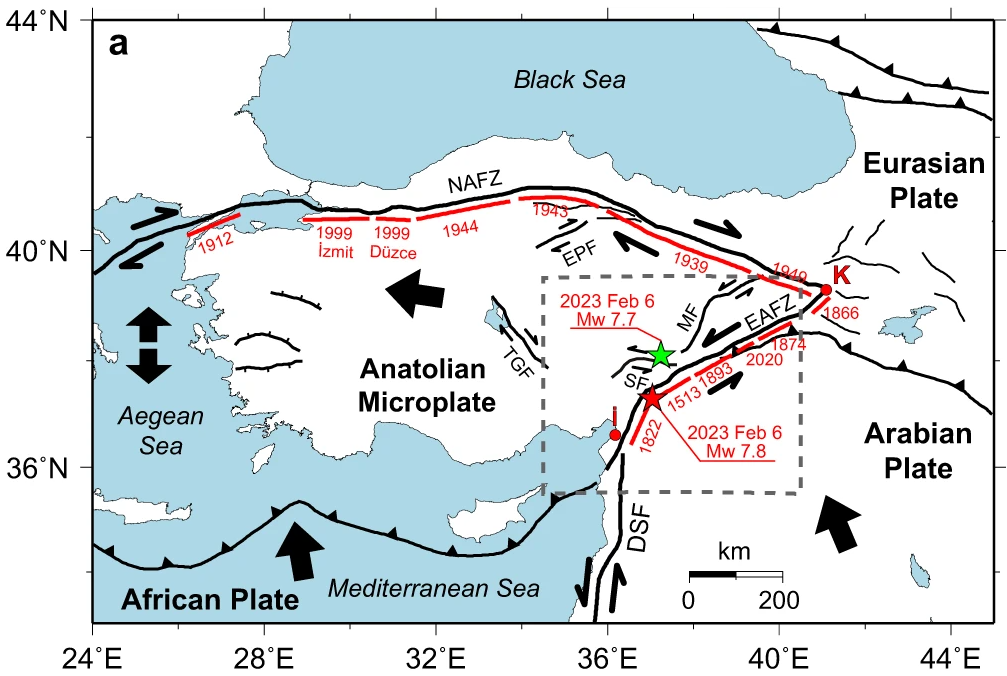
\includegraphics[width=.54\textwidth]{figures/eqturk23_tect.png}
  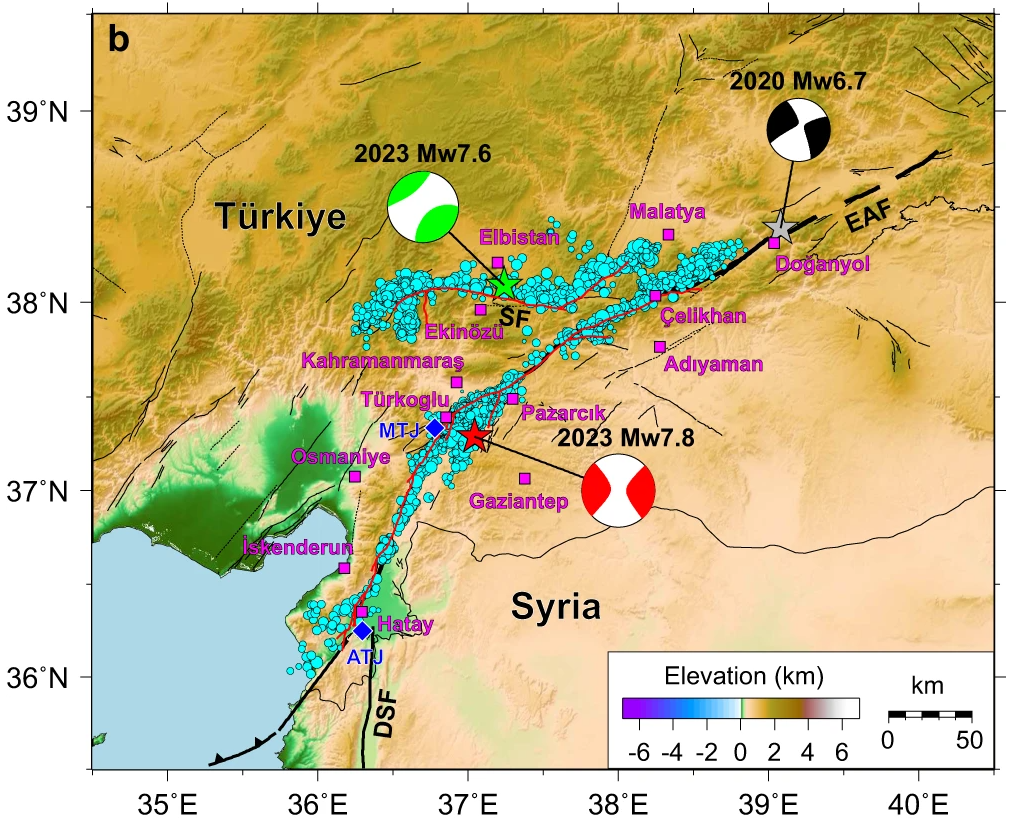
\includegraphics[width=.44\textwidth]{figures/eqturk23_fm.png}
\end{center}
    \caption{Tectonic backround (a) and Focal mechanisms (b) of 2023 Turkey earthquake doublet \cite{Liu_2023}.}
    \label{fig:proc-net}
\end{figure} 
\end{block}
%------------------------------------------------
%    SOFTWARE DESING
%------------------------------------------------
\begin{block}{GNSS Network \& Data processing}
{\small
Data from 57 continuously operating GNSS stations in distances ranging from 800km to 1400km from the epicenter were analyzed.\\
\textbf{Station Equipment:}
\begin{itemize}\setlength\itemsep{.3em}
  \item Receiver type: LEICA\\
    (most of them GR30, also GRX1200GGPRO / GRX1200+GNSS)
  \item Antenna type LEICA\\
    LEIAR10 / LEIAS10 (few stations: LEIAX1202GG)
  \item Observation interval: 1s
\end{itemize}

\textbf{Processing scheme:}
\begin{itemize}\setlength\itemsep{.3em}
  \item Precise Point Positioning with Ambiguity Resolution using PRIDE-PPPAR Software \cite{Geng_2019}.
  \item Satellite systems: GPS / GLO / GAL / BDS-2/3
  \item Elevation angle: 7 deg
  \item Kinematic mode
  \item Reference Frame: IGS20
  \item Final IGS Products for satellite
  \item ANTEX File: IGS20\_2247
  \item Tropospheric modeling: VMF1
\end{itemize}

%Precise Point Positioning w Ambiguity Resolution
%
%Sat systems:
%
%GPS / GLO / GAL / BDS-2/3
%
%Elevation angle: 7 deg
%
%--Kinematic mode
%
%Reference Frame: IGS20
%
%Final IGS Products for satellite:
%
%- Orbits (.SP3)
%
%- Clocks (.CLK)
%
%- Earth Orientation Parameters (.ERP)
%
%- Attitude (.OBX)
%
%- Bias (.BIA)
%
%ANTEX File: IGS20\_2247
%
%For Tropospheric modeling: VMF1
}
%\begin{center}
%  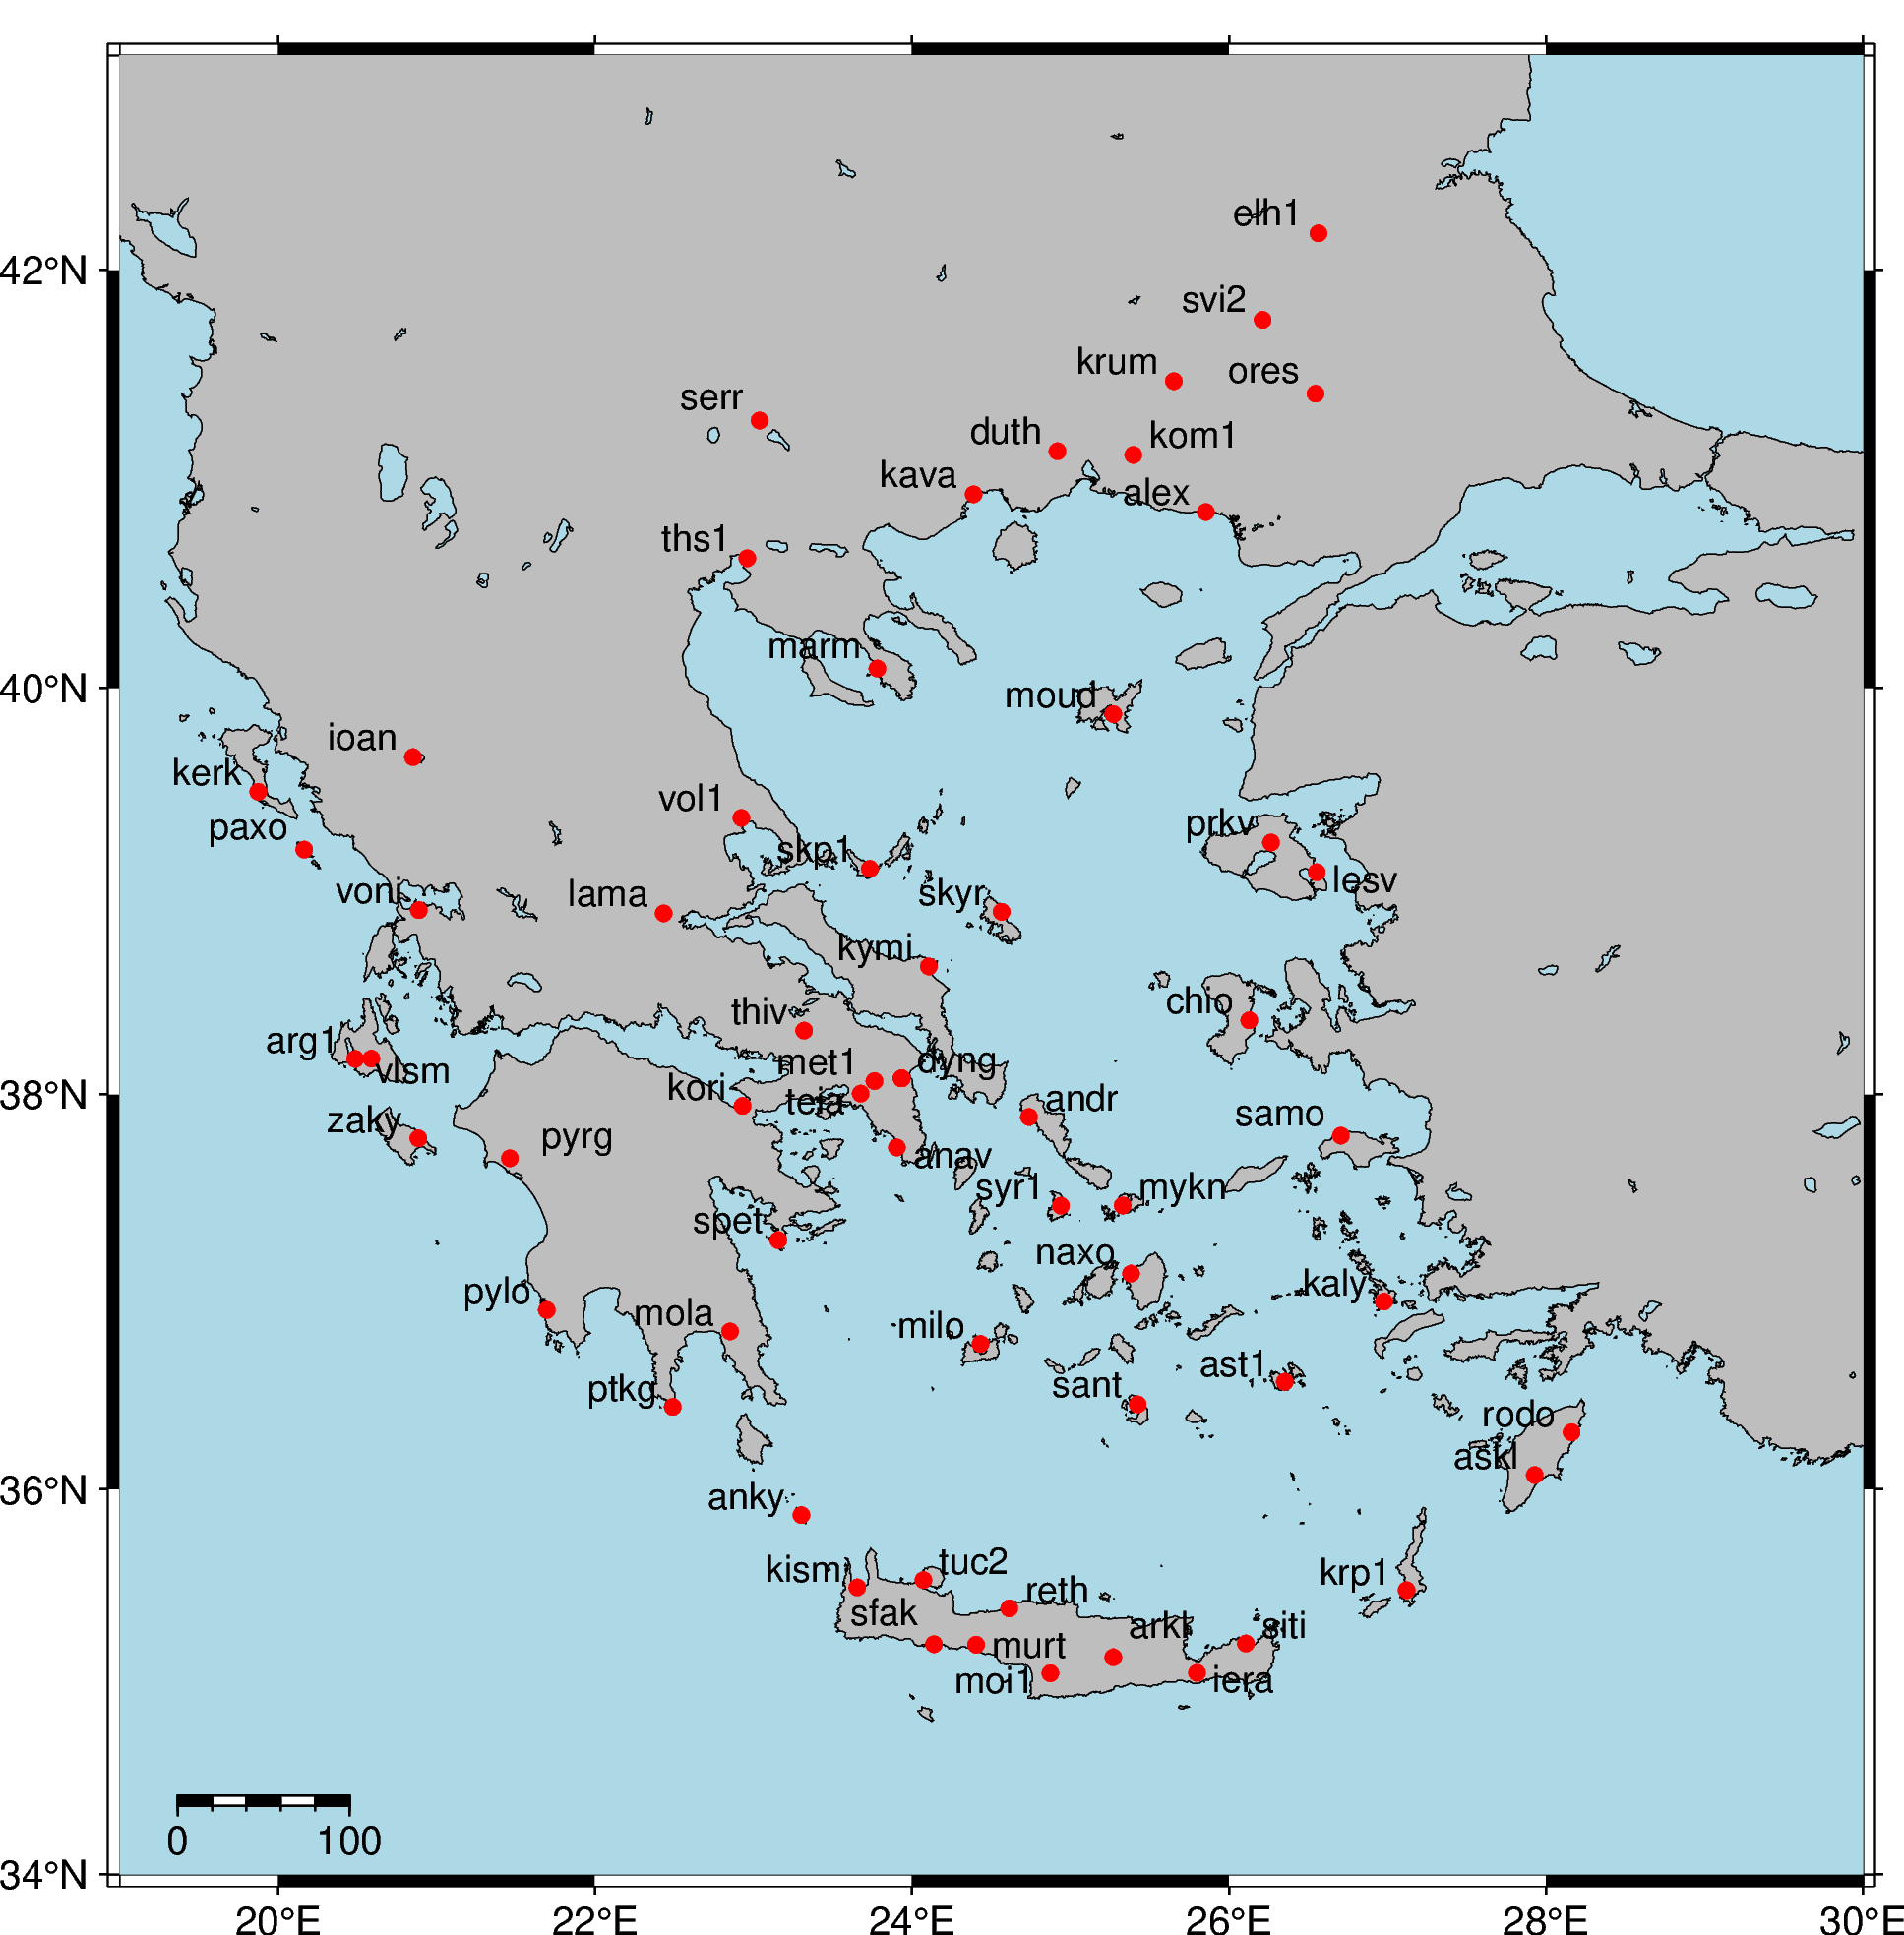
\includegraphics[width=.97\textwidth]{figures/gnss_network.png}
%\end{center}
%\vspace*{48cm}

\begin{figure}
\begin{center}
  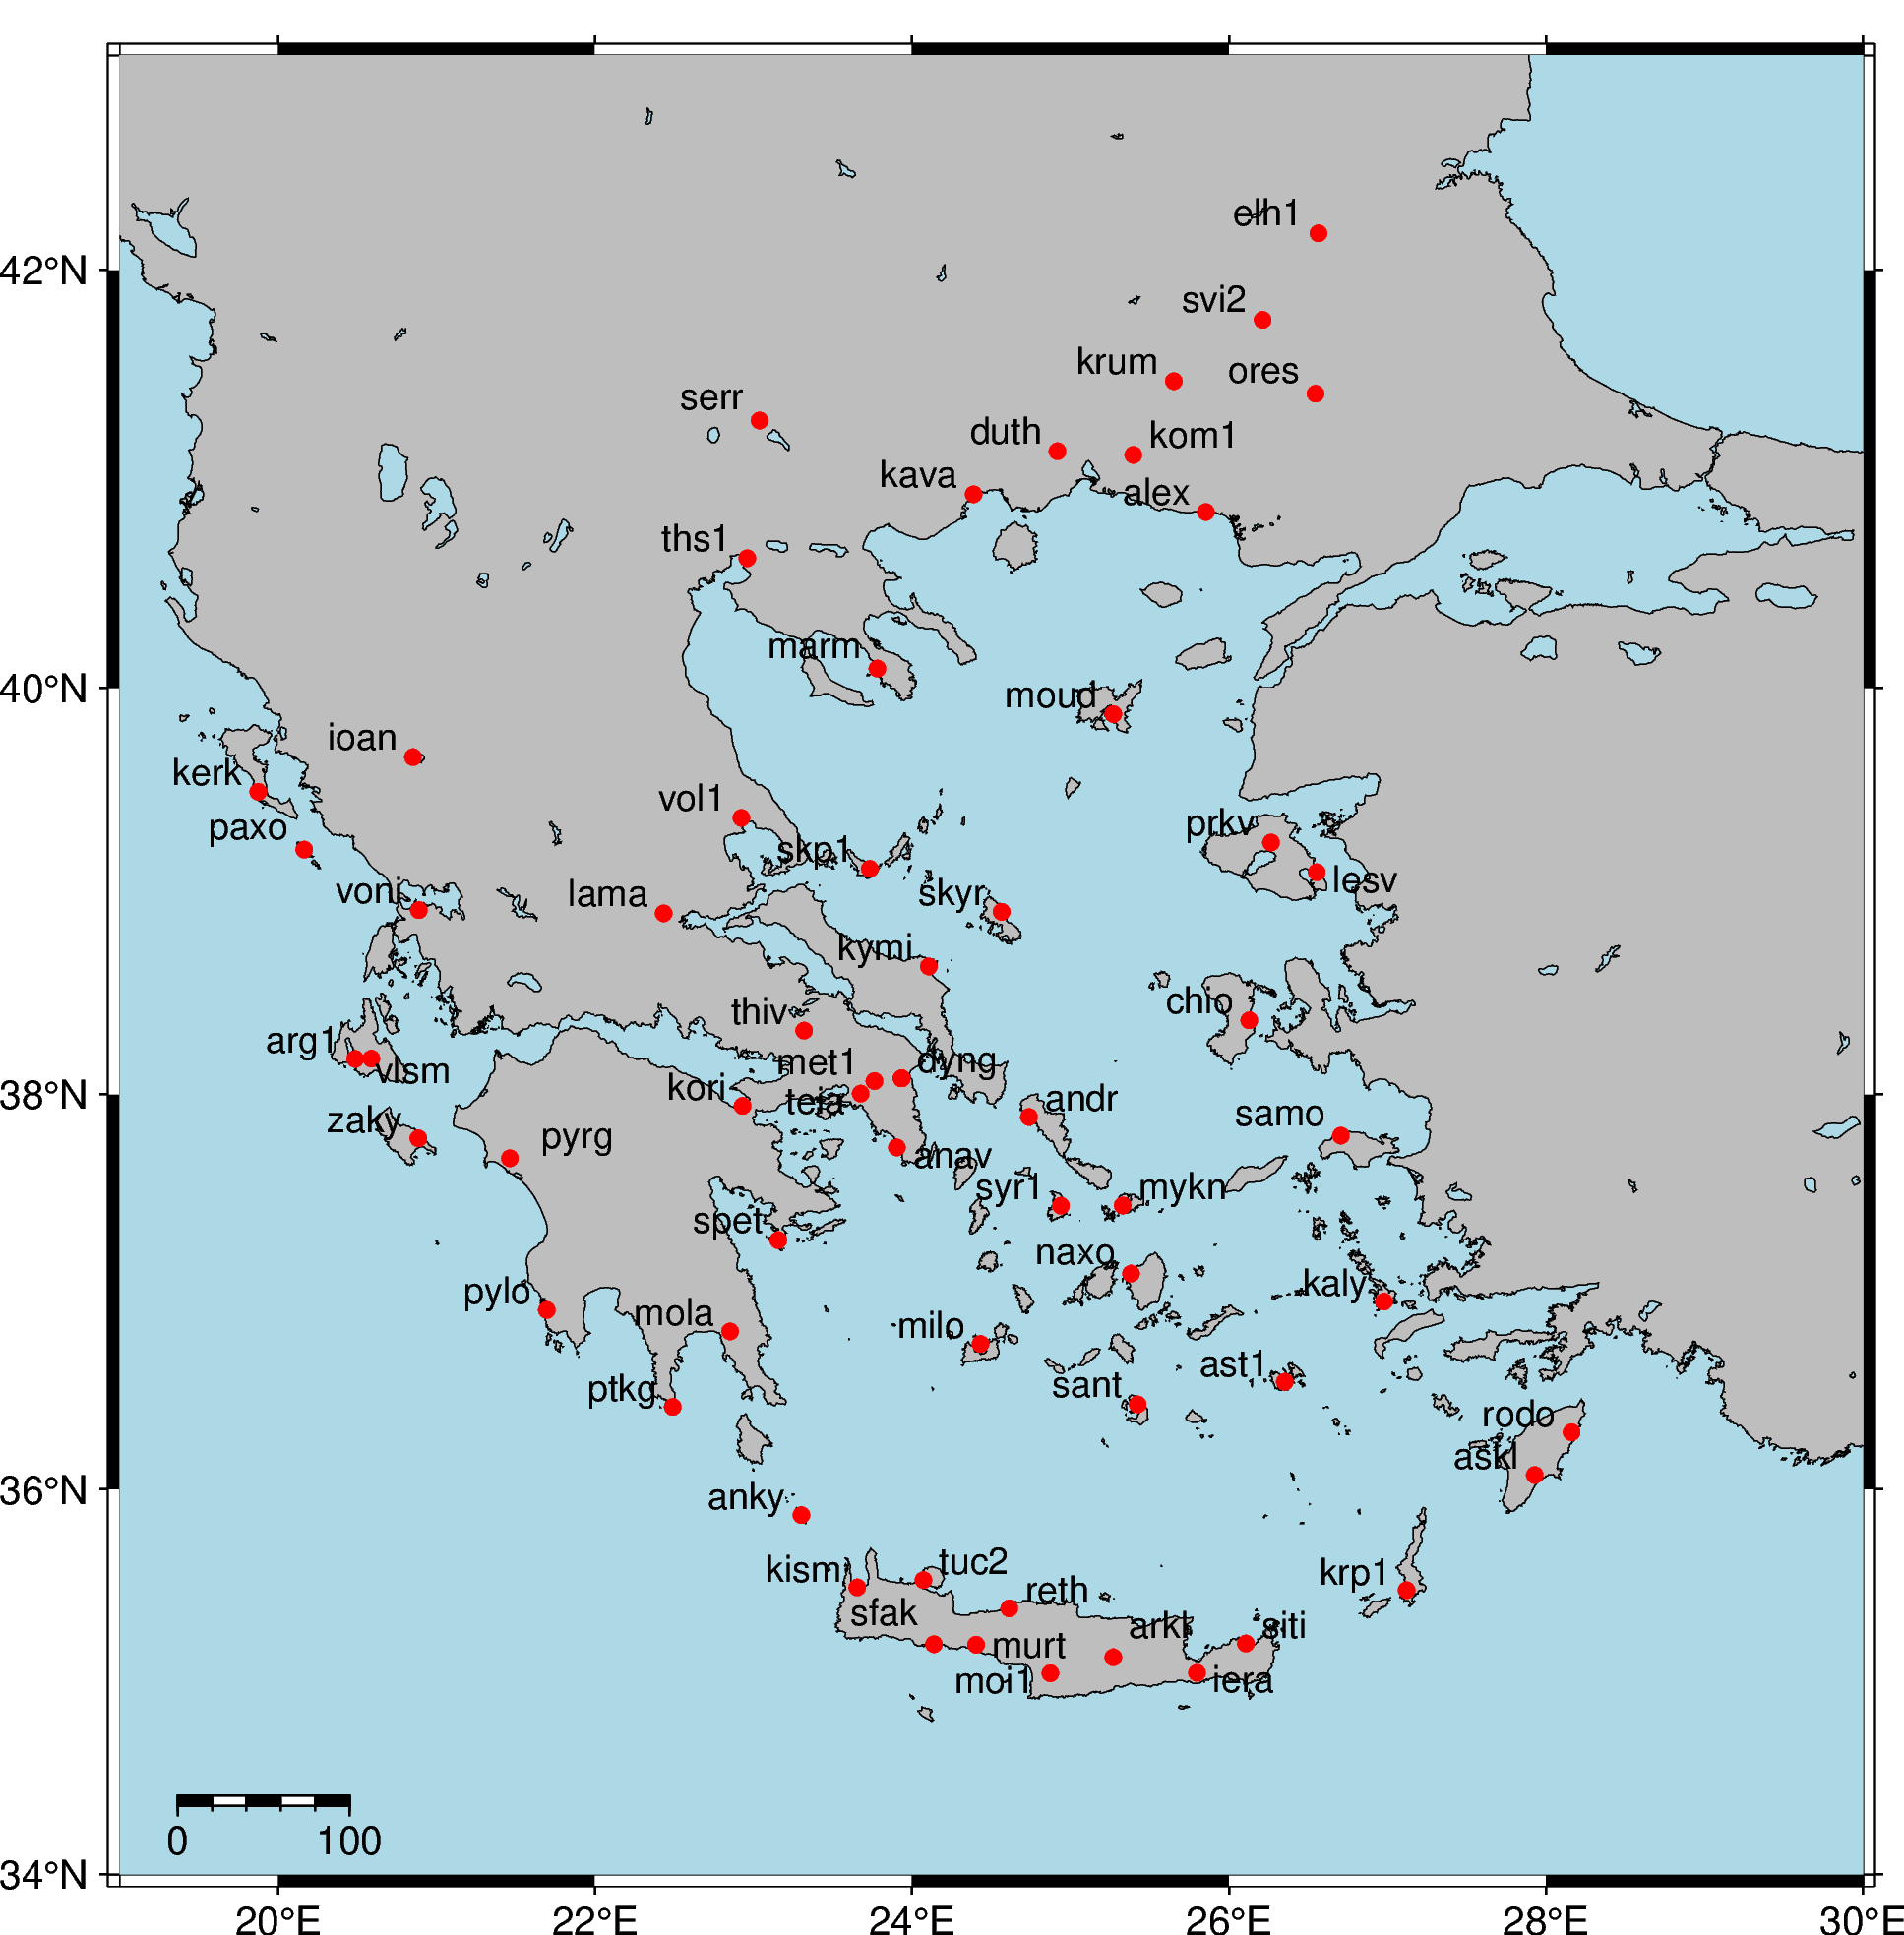
\includegraphics[width=.75\textwidth]{figures/gnss_network.png}
\end{center}
    \caption{Distribution of permanent GNSS stations analyzed.}
    \label{fig:proc-net}
\end{figure} 
\begin{center}
\vskip-.5cm
{\footnotesize \textbf{Acknowledgments} to Metrica SA for the free availability of the 1Hz GNSS data of HxGN SmartNet for this study.}
\hspace*{1cm}
  
\includegraphics[width=.4\textwidth]{logo_HXgn.png}
  
\includegraphics[width=.2\textwidth]{logo_metrica.png}
\end{center}     
\end{block}
%\bigskip
%\begin{alertblock}{Contact Information}
%\begin{itemize}
%\item Web: \href{http://dionysos.survey.ntua.gr}{dionysos.survey.ntua.gr}
%\item Email: \href{xanthos@mail.ntua.gr}{xanthos@mail.ntua.gr}
%\end{itemize}
%\end{alertblock}

%\vfill
%----------------------------------------------------------------------------
%	CONTACT INFORMATION
%----------------------------------------------------------------------------
%\setbeamercolor{block alerted title}{fg=black,bg=norange} % Change the alert block title colors
%\setbeamercolor{block alerted body}{fg=black,bg=white} % Change the alert block body colors
\vskip-1.5cm
\begin{minipage}{\threecolwid}
  \begin{column}{\twocolwid}
		\vspace*{1.0\baselineskip}
		\begin{center}
		  
\includegraphics[width=.97\textwidth]{figures/ESC2024_webheader.png}
		\end{center}
  \end{column}
%  \begin{column}{.1\sepwid}\end{column}
  \begin{column}{\onecolwid}
  \vspace*{1.0\baselineskip}
    \begin{alertblock}{Contact Information}
    {\small
  		\begin{itemize}
	  		\item P. Psimoulis (\href{Panagiotis.Psimoulis@nottingham.ac.uk}{Panagiotis.Psimoulis@nottingham.ac.uk})
		  	\item D. Anastasiou (\href{danastasiou@mail.ntua.gr}{danastasiou@mail.ntua.gr})
		  \end{itemize}
		  }
  	\end{alertblock}
  \end{column}
\end{minipage}

%
%\begin{alertblock}{Contact Information}
%\begin{itemize}
%\item Web: \href{http://dionysos.survey.ntua.gr}{dionysos.survey.ntua.gr}
%\item Email: \href{xanthos@mail.ntua.gr}{xanthos@mail.ntua.gr}
%\end{itemize}
%\end{alertblock}



%-----------------------------------------------------------------------------

\end{column} % End of the first column
%\vrule{}

% Empty spacer column
\begin{column}{\sepwid}\end{column}

% Begin a column which is two columns wide (column 2)
\begin{column}{\twocolwid} 

%--------------------------------------------------------------------------
%	PROCESSING
%---------------------------------------------------------------------------

\begin{block}{Data Analysis}

{\small
The low-frequency noise of the gnss stations which could be due to various error sources (multipath error, unmitigated troposphere effect, etc.), potential seismic displacement of the gnss stations was masked. Since no co-seismic displacement was expected at the stations (>800km distance from epicentres), we applied a high-pass 'Butterworth' filter with cut-off frequency of 0.1Hz to remove any low-frequency noise of the gnss data and without affecting significantly the potential dynamic displacement of the gnss stations.

The time interval of the transient seismic response of each gnss was defined with starting time the time of the seismic event plus the required time of P-waves (with velocity of 6km/s) to travel at the respective gnss station and covering a period of 400 seconds to ensure that all the transient response is captured.

For the defined period, the Peak Ground Displacemet of neu was defined as the max values of the respective time-series.

For the noise level estimation of the filtered neu time-series, we computed the standard deviation for the 10-minute period before the first seismic event. We defined as the noise level, the rather conservative 3$\sigma$ value to ensure that any potential response larger than this threshold corresponds to the transient seismic response.
}


\begin{figure}
\begin{center}
  \fbox{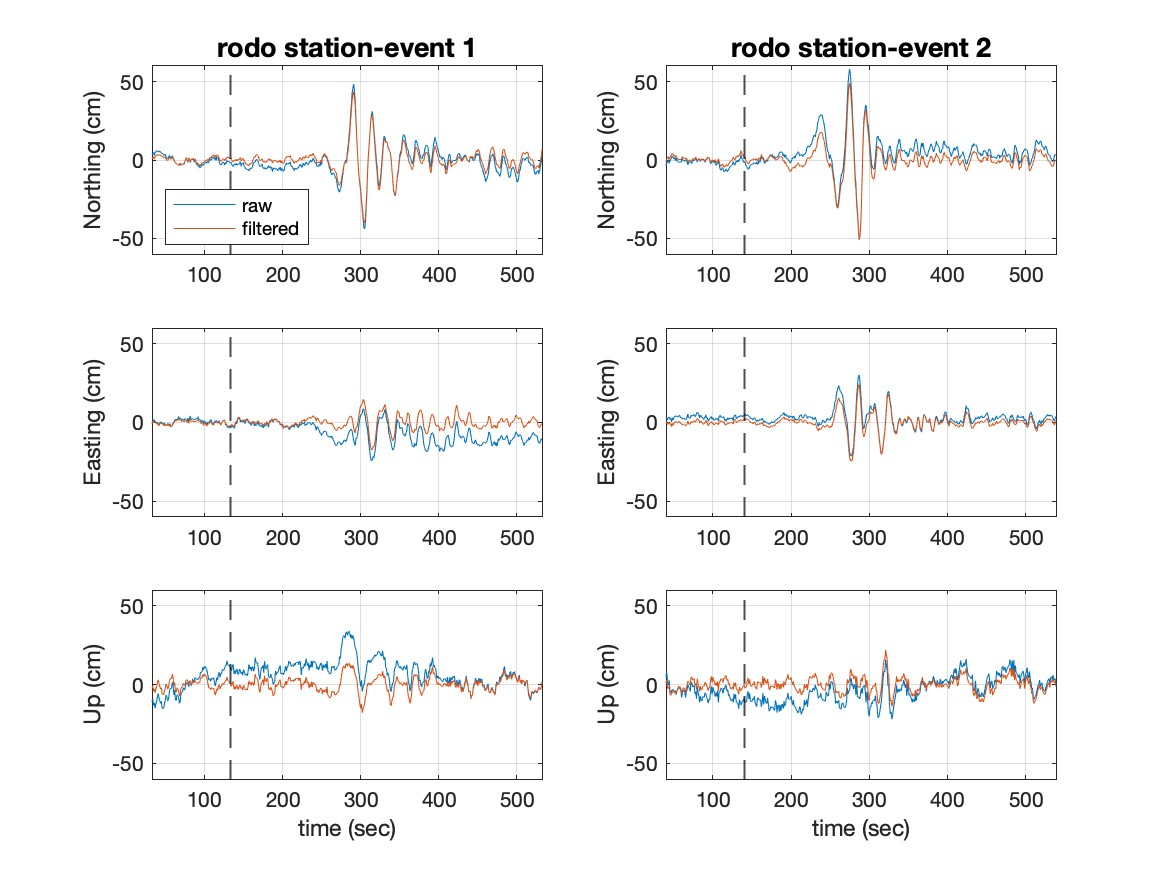
\includegraphics[width=.32\textwidth]{figures/rodo_NEU_nofilter_vs_filtered_010.jpg}}
  \textcolor{blue!40}{\vrule width 1pt}
  \fbox{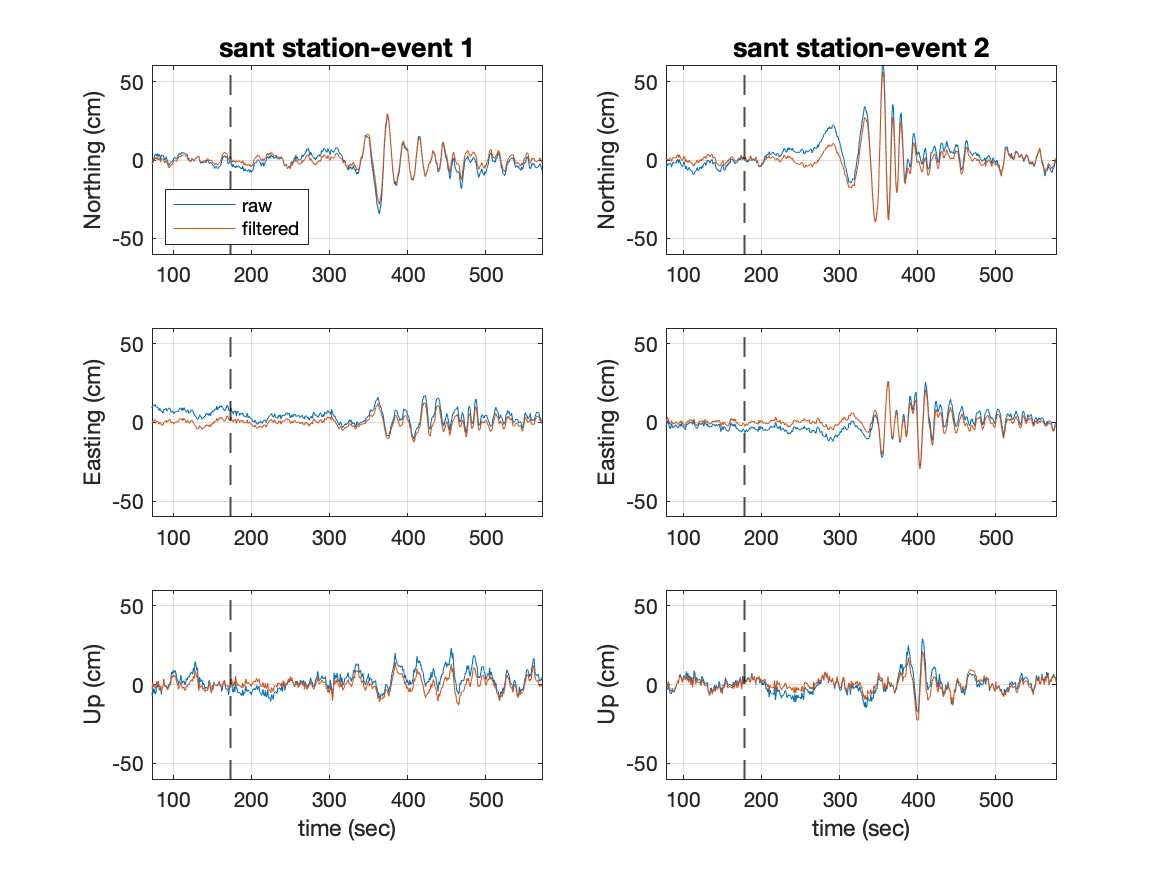
\includegraphics[width=.32\textwidth]{figures/sant_NEU_nofilter_vs_filtered_010.jpg}}
  \textcolor{blue!40}{\vrule width 1pt}
  \fbox{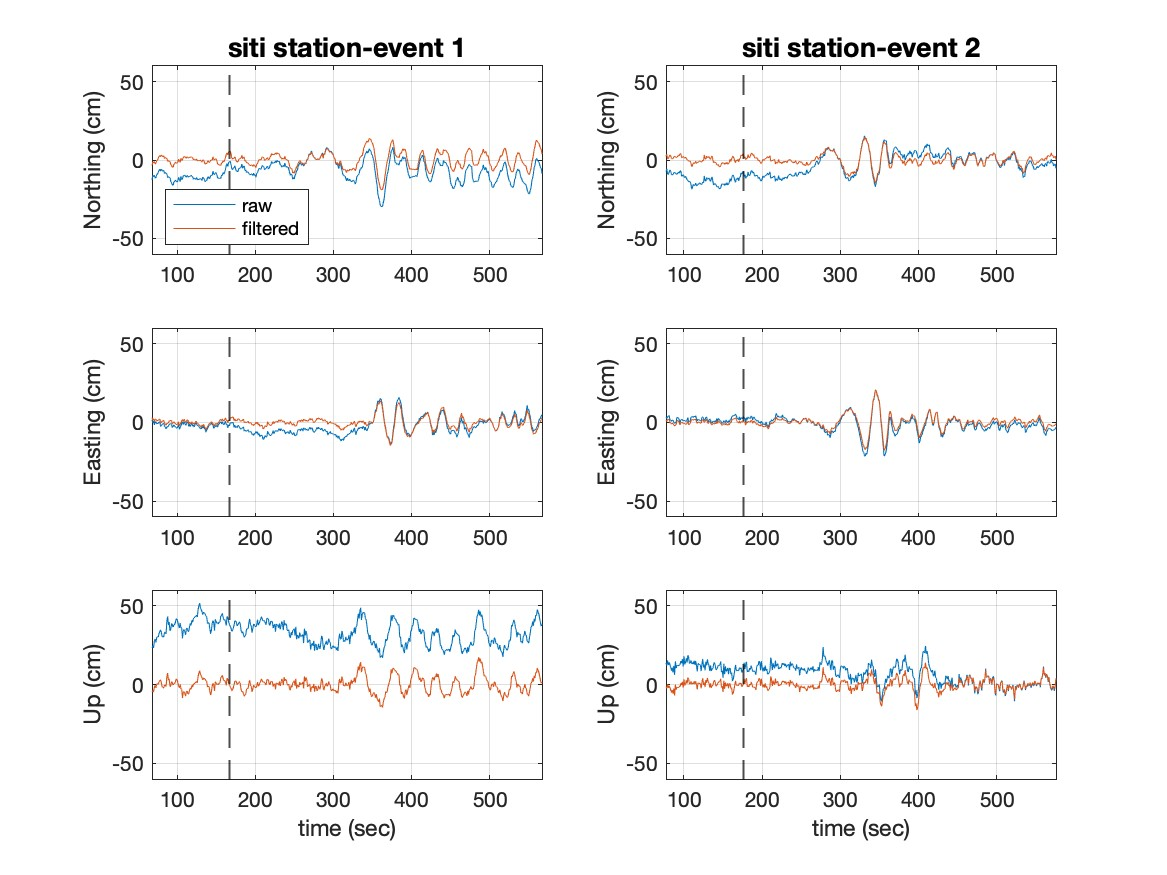
\includegraphics[width=.32\textwidth]{figures/siti_NEU_nofilter_vs_filtered_010.jpg}}
\end{center}
\vskip-1cm
\textcolor{blue!40}{\rule{\textwidth}{1pt}}\\
\begin{center}
  \fbox{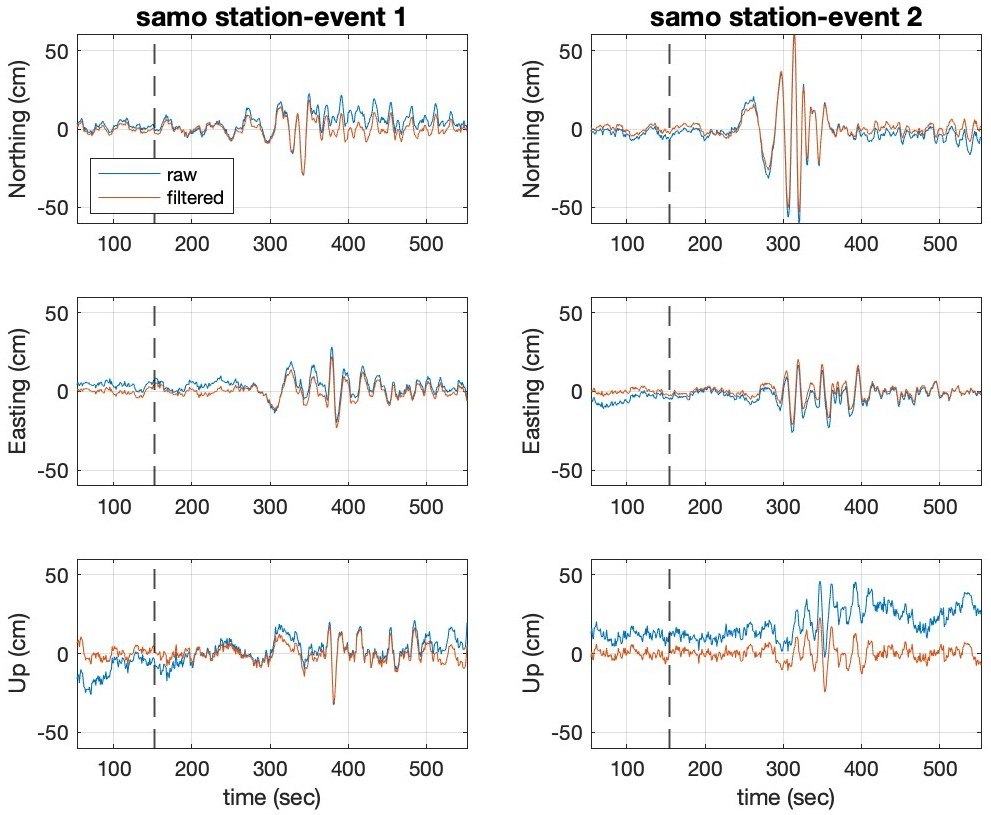
\includegraphics[width=.32\textwidth]{figures/samo_NEU_nofilter_vs_filtered_010.jpg}}
  \textcolor{blue!40}{\vrule width 1pt}
  \fbox{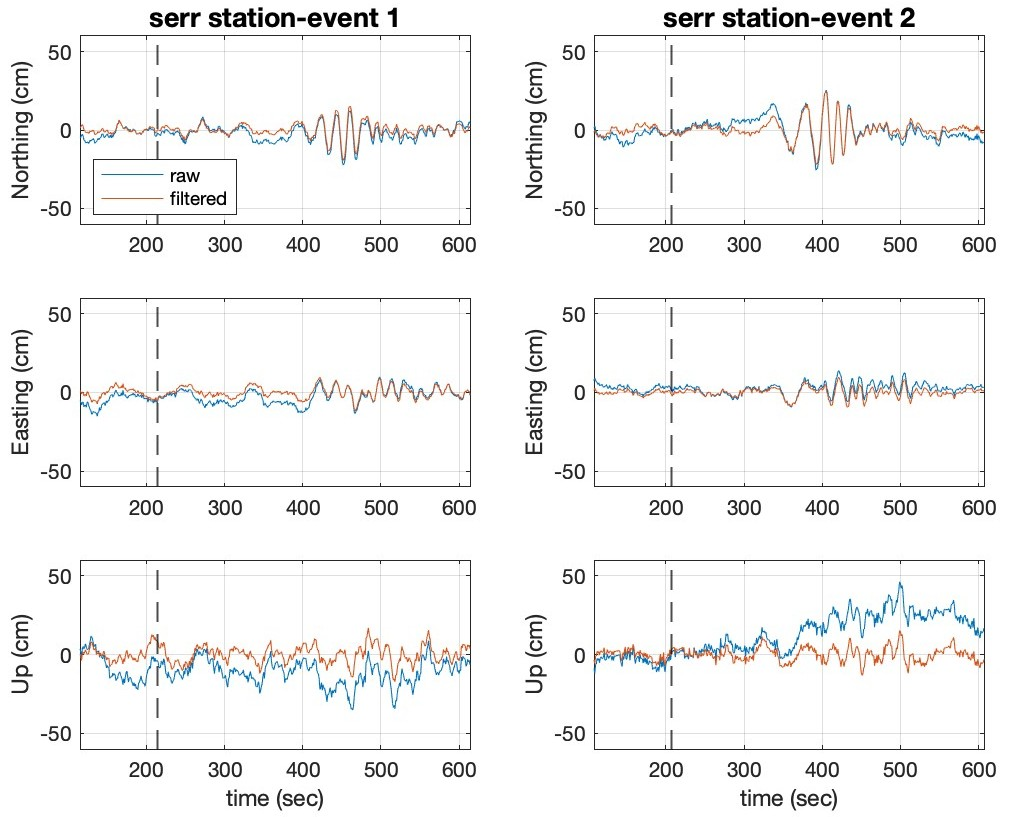
\includegraphics[width=.32\textwidth]{figures/serr_NEU_nofilter_vs_filtered_010.jpg}}
  \textcolor{blue!40}{\vrule width 1pt}
  \fbox{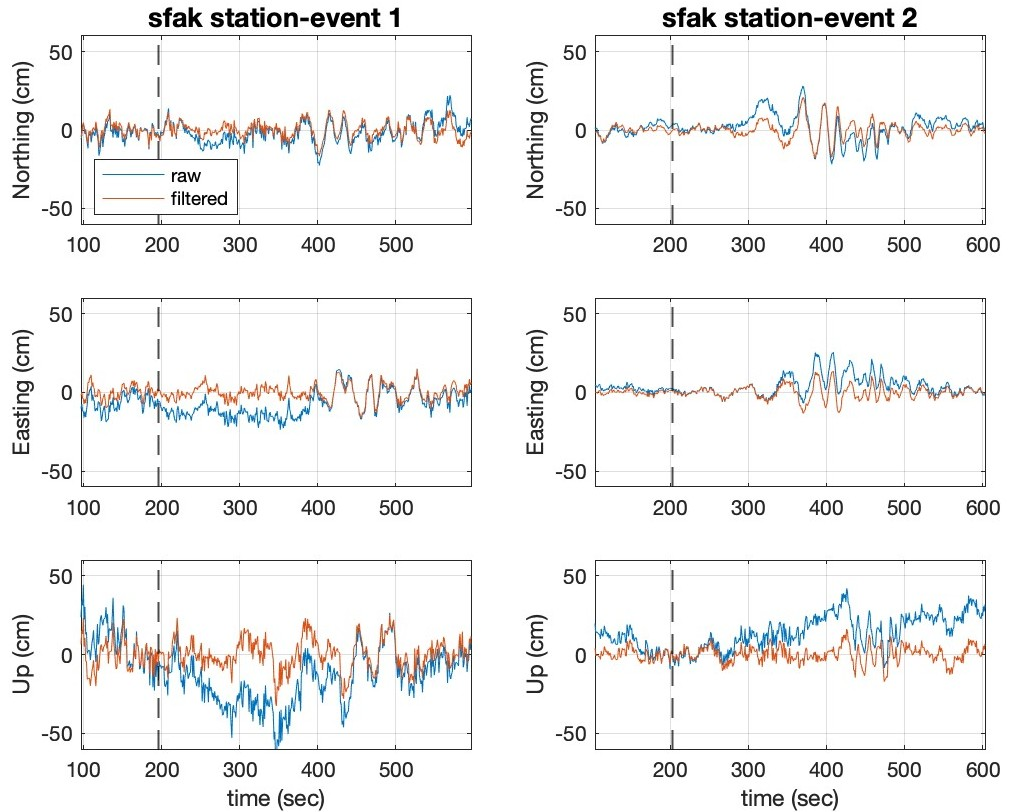
\includegraphics[width=.32\textwidth]{figures/sfak_NEU_nofilter_vs_filtered_010.jpg}}
\end{center}
    \caption{Raw and filtered time series analysis for six (6) stations.}
    \label{fig:proc-net}
\end{figure}      

%\begin{figure}
%\begin{center}
%  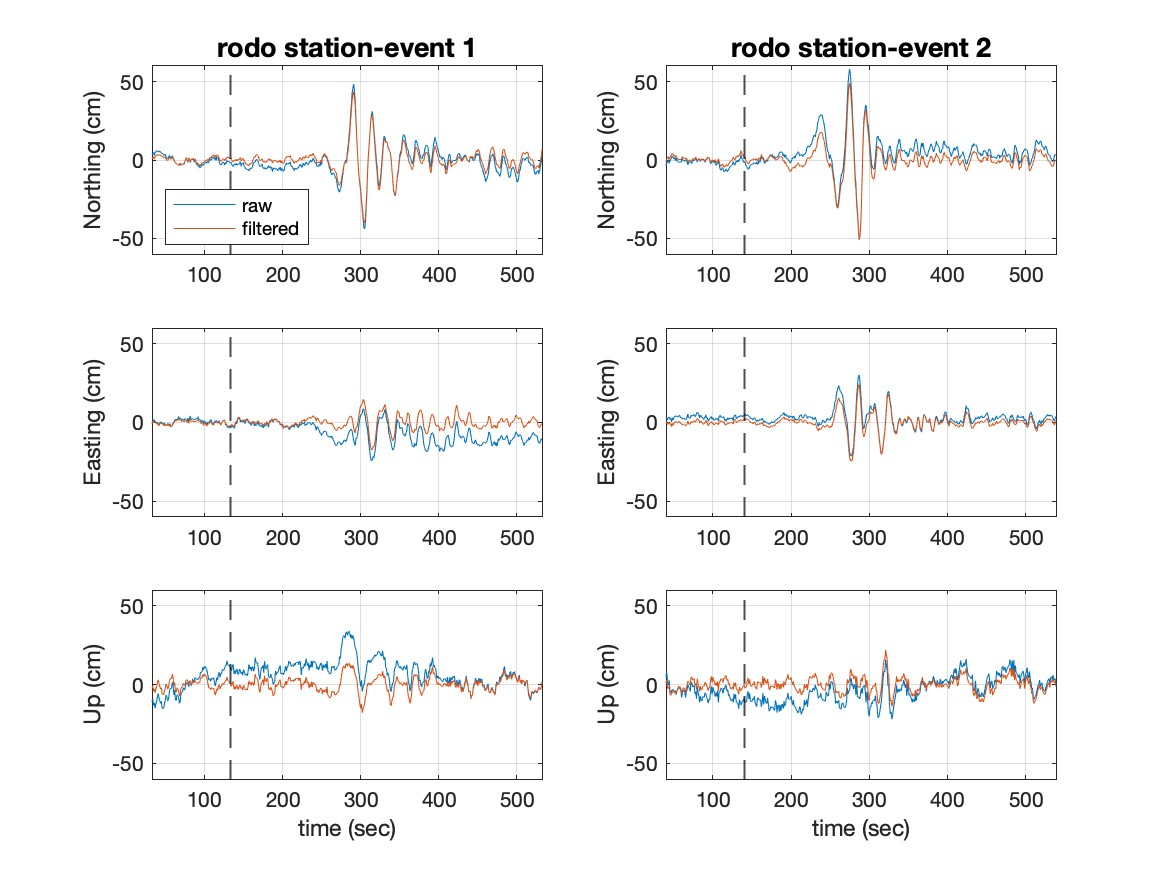
\includegraphics[width=.47\textwidth]{figures/rodo_NEU_nofilter_vs_filtered_010.jpg}
%  \textcolor{blue!40}{\vrule width 1pt}
%  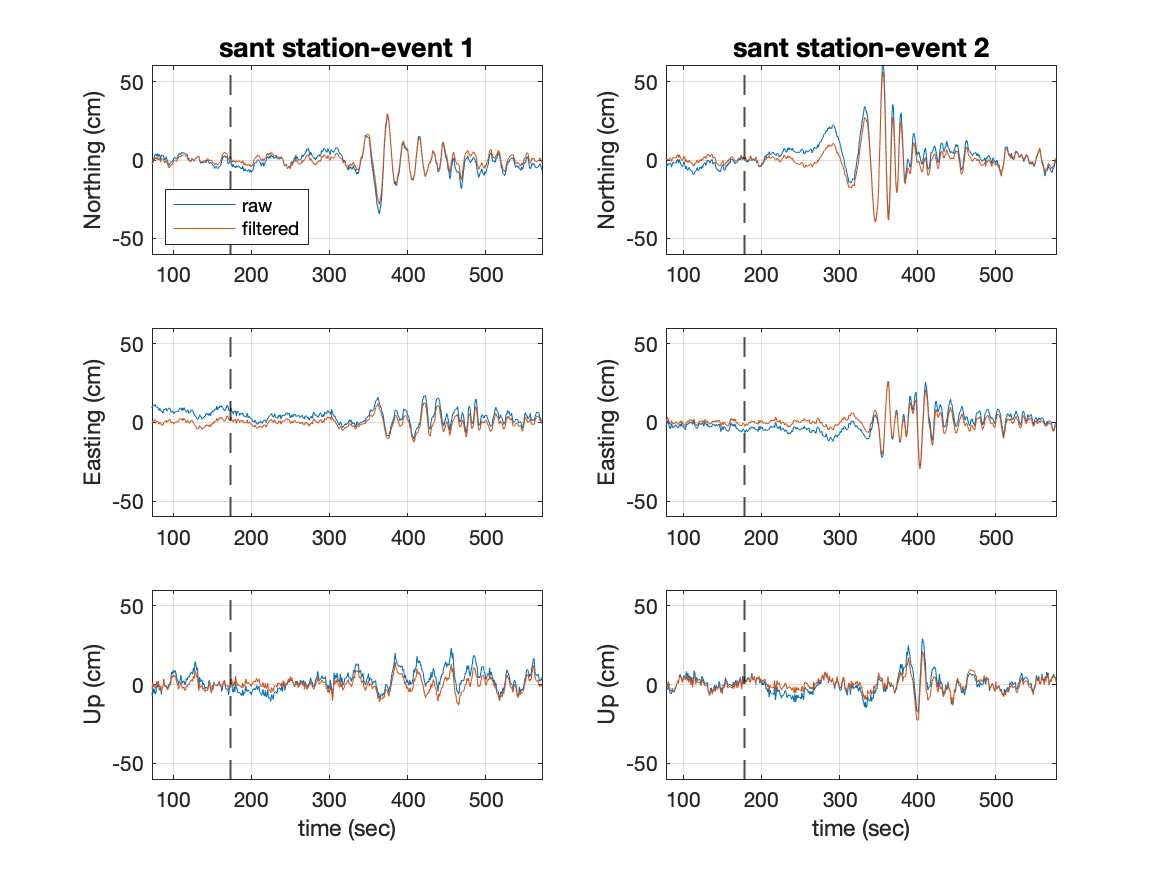
\includegraphics[width=.47\textwidth]{figures/sant_NEU_nofilter_vs_filtered_010.jpg}
%%  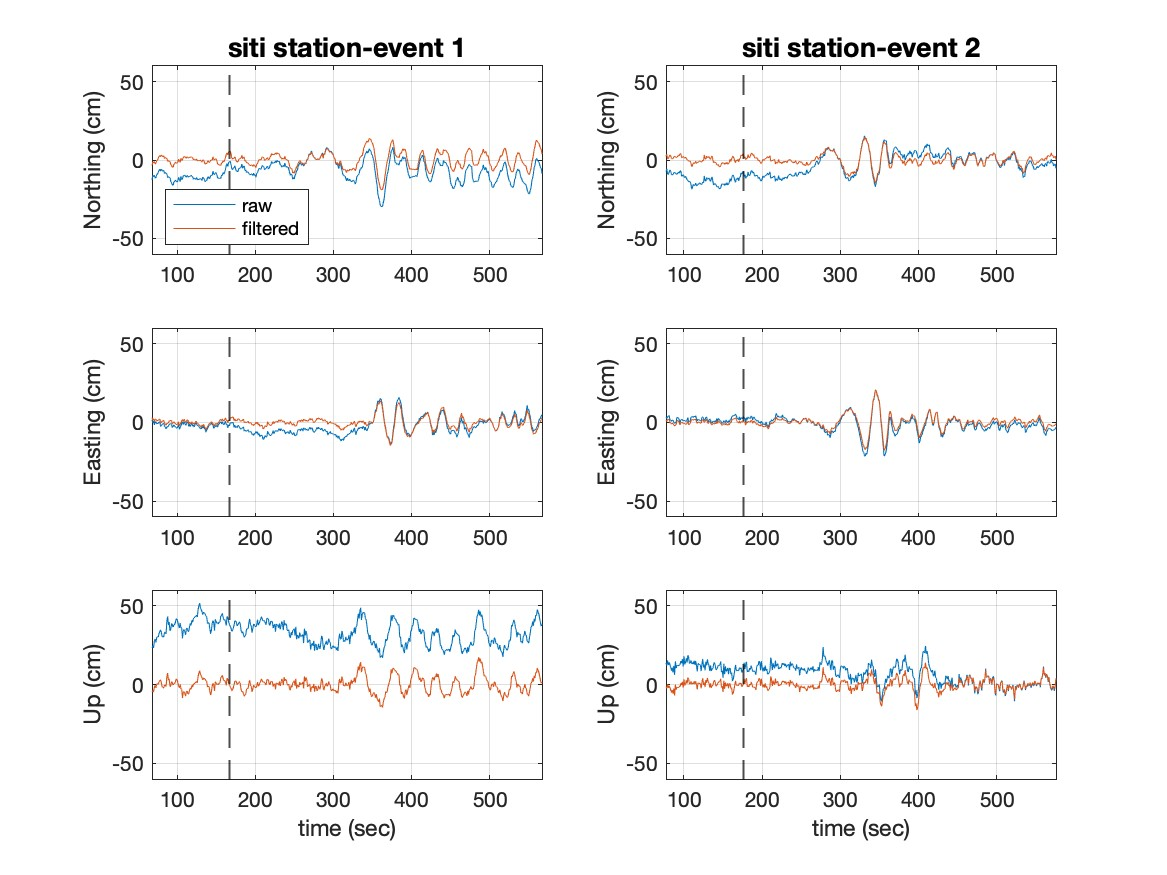
\includegraphics[width=.32\textwidth]{figures/siti_NEU_nofilter_vs_filtered_010.jpg}
%\end{center}
%\textcolor{blue!40}{\rule{\textwidth}{1pt}}\\
%\begin{center}
%  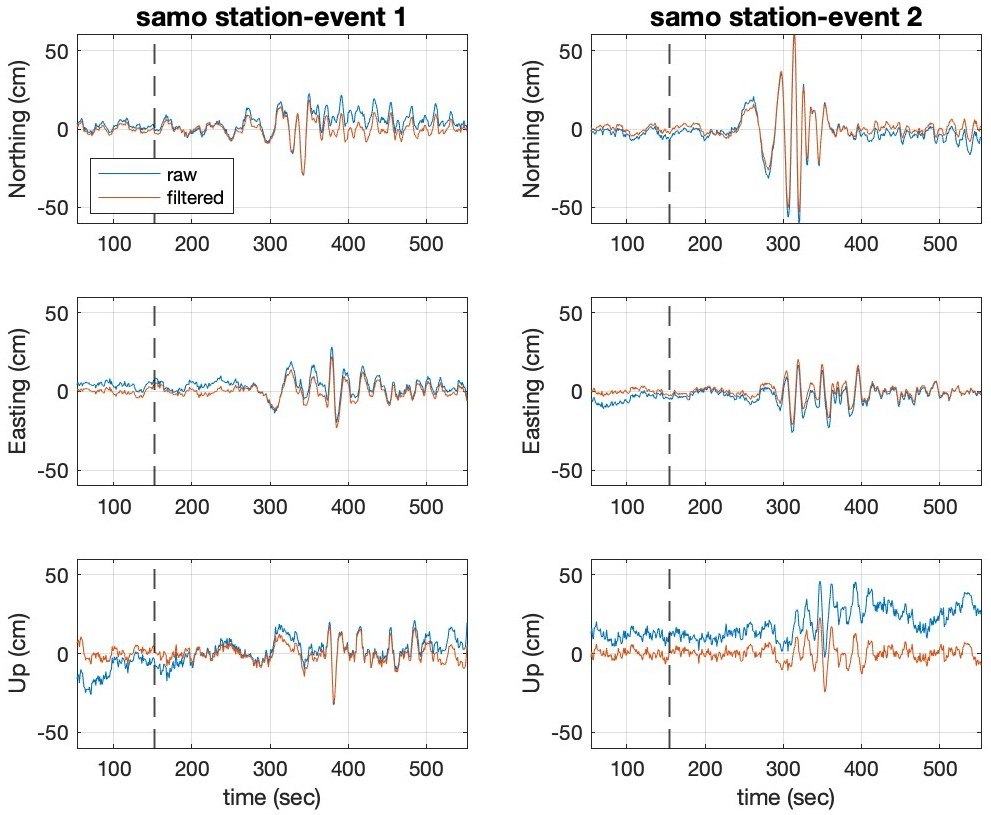
\includegraphics[width=.47\textwidth]{figures/samo_NEU_nofilter_vs_filtered_010.jpg}
%  \textcolor{blue!40}{\vrule width 1pt}
%  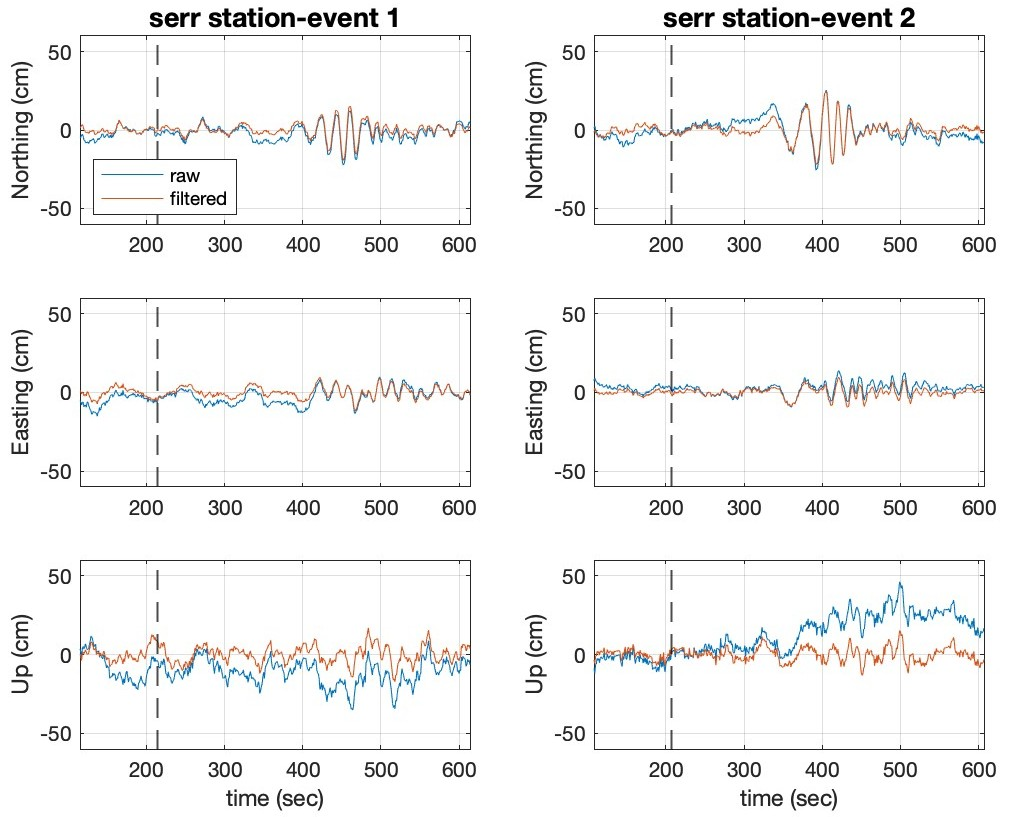
\includegraphics[width=.47\textwidth]{figures/serr_NEU_nofilter_vs_filtered_010.jpg}
%%  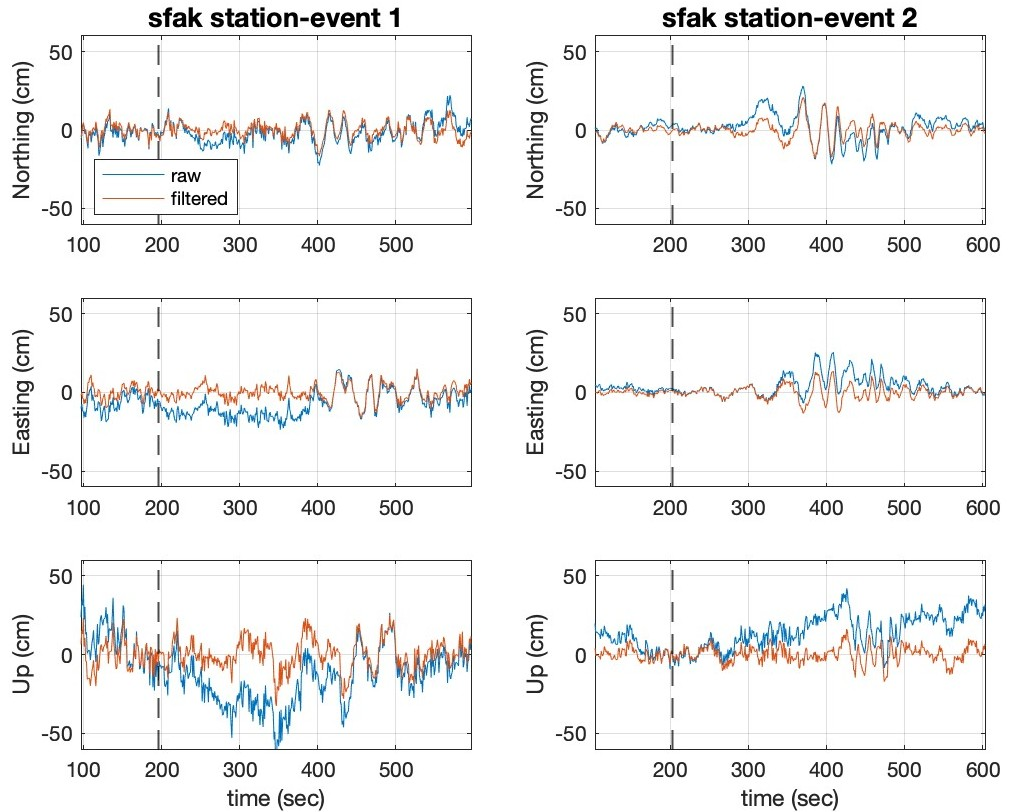
\includegraphics[width=.32\textwidth]{figures/sfak_NEU_nofilter_vs_filtered_010.jpg}
%\end{center}
%    \caption{Processed stations.}
%    \label{fig:proc-net}
%\end{figure}      
\end{block}


%-------------------------------------------------------------------------
%	PRELIMINARY RESULTS
%-------------------------------------------------------------------------
%\begin{block}{Preliminary Results}
%{\small
%\end{block}
%-----------------------------------------------------------------------------

\vskip-3cm
\begin{columns}[t]
\begin{column}{\onecolwid}
\begin{block}{}
	\begin{figure}
	\begin{center}
	\vskip.2cm
	  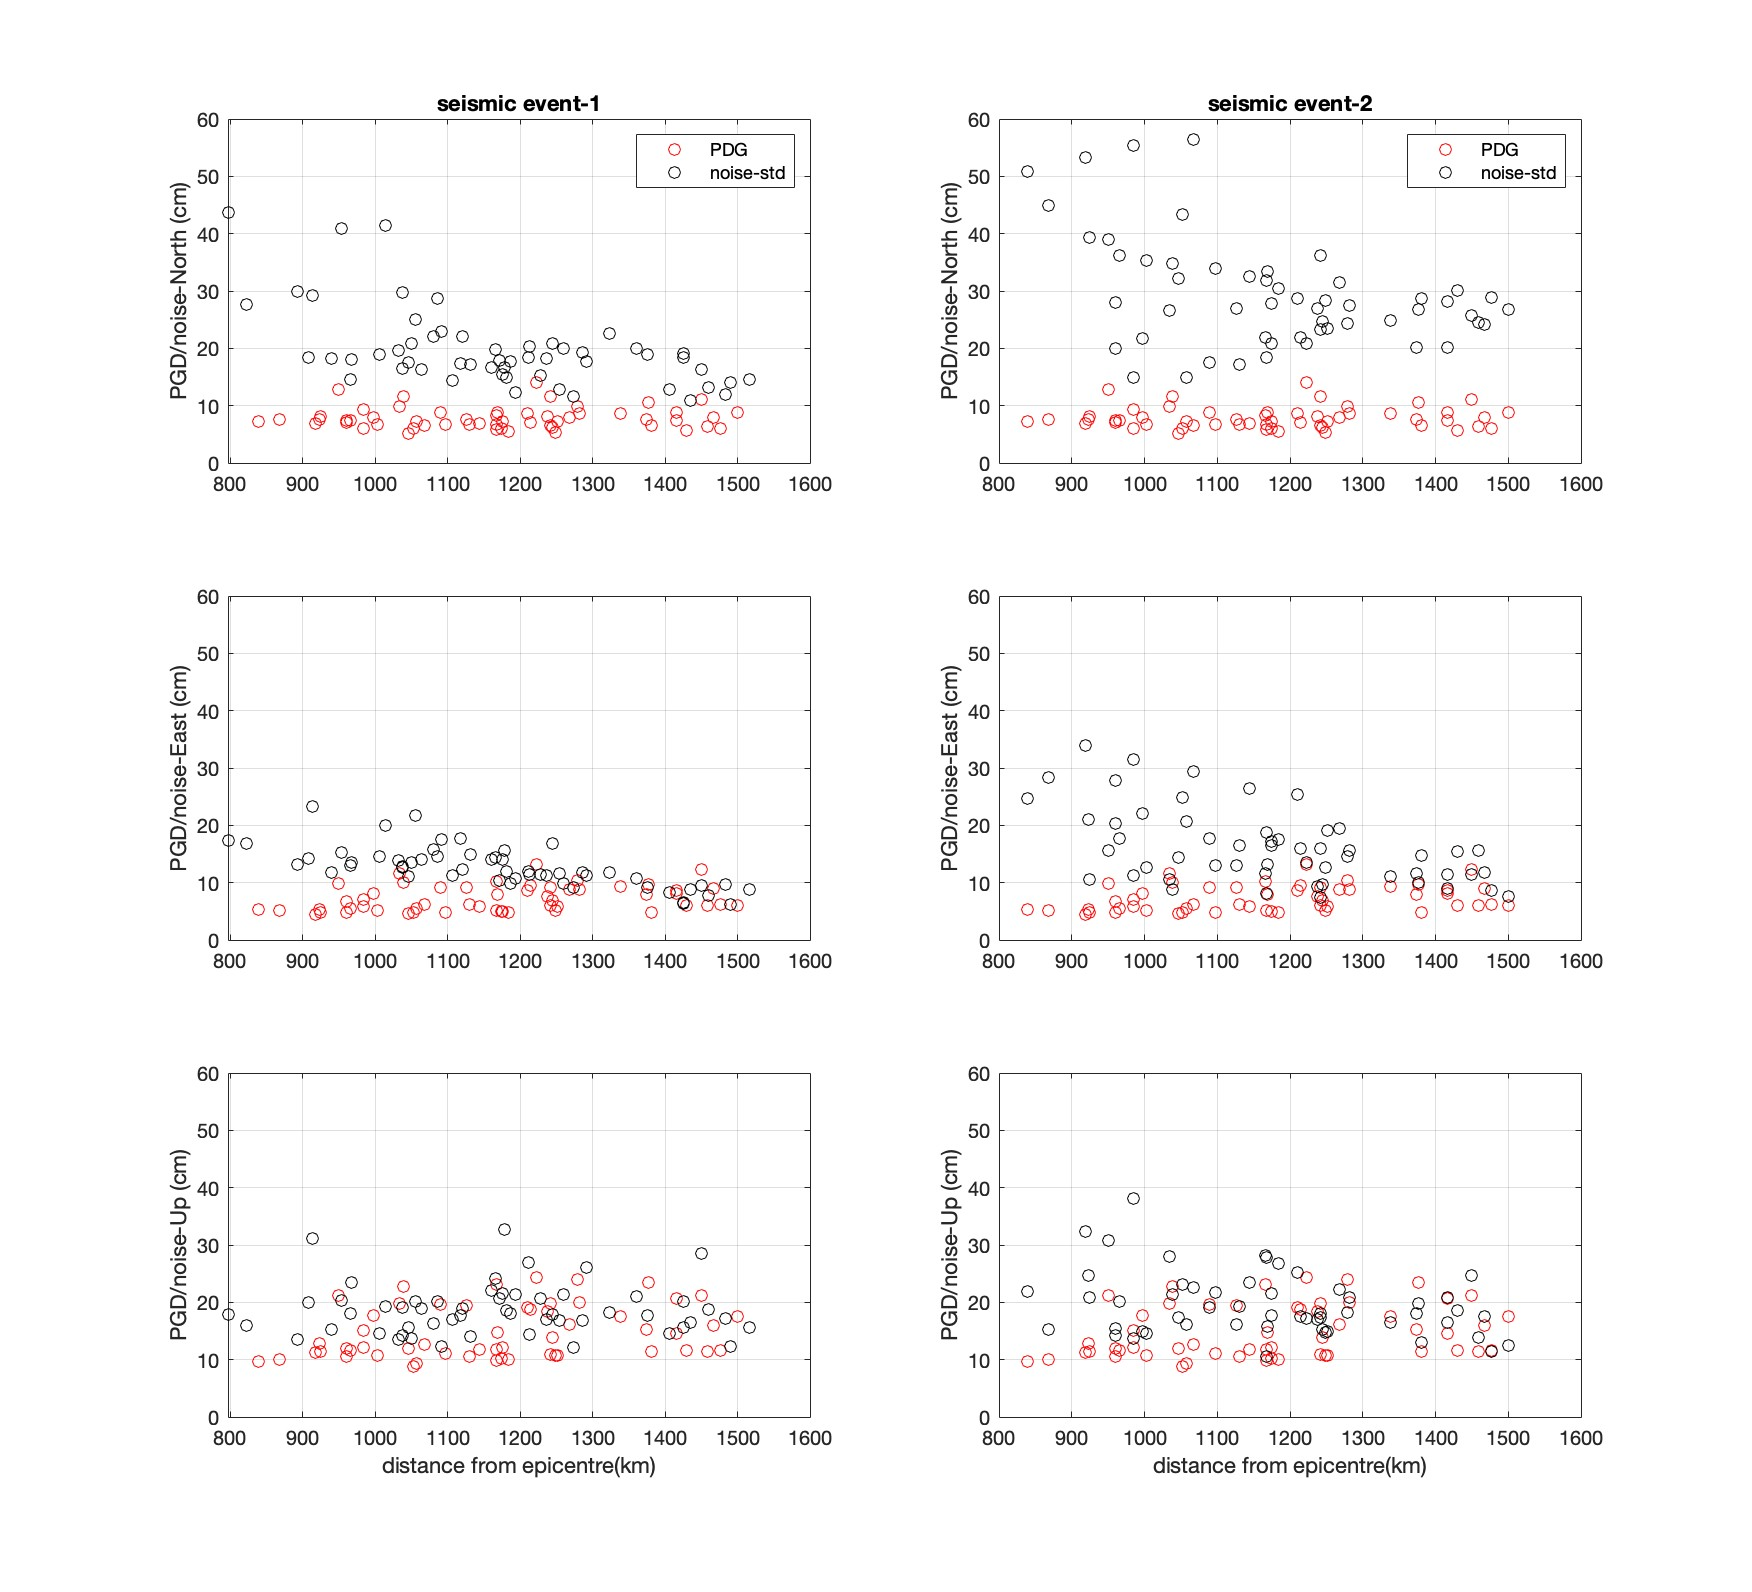
\includegraphics[width=.97\textwidth]{figures/PGD_maxnoise_vs_distance_2.jpg}
	\end{center}
	    \caption{Diagrams of PGD maximum noise vs distance of all the stations for the two seismic events.}
	    \label{fig:proc-net}
	\end{figure}      
\end{block}
\end{column}


\begin{column}{\sepwid}\end{column} % Empty spacer column

\begin{column}{\onecolwid}
\begin{block}{Discussion}
{\small

From the first analysis of the PGD values the following points are observed:

\begin{itemize}\setlength\itemsep{1em}
  \item For both seismic events, in the northing component is observed the highest values of PGD indicating that the this direction is affacted by the propagation of the seismic waves.
  \item The second seismic event has larger far-field impact probably due to the geometry of the seismic fault and the directivity of the seismic waves propagation.
  \item The Up component is not affacted by the seismic events potentially due to the small impact that the S-waves may have for far-field stations.
  \item The PGD values tend to rdecrease with the distance from the epicetres. ?However it is obvious the impact of the directivity of the propagation of the seismic waves and the orientation of the seismic faults, as the PGD values of gnss stations of similar distance from the epicentres has large range. For instance, the PGD values of the northing component of gnss stations with ~1000km epicentre distance for the second seismic event range between 20 to 60cm.
\end{itemize}
}



\end{block}
\end{column}
\end{columns}

%----------------------------------------------------------------------------------------
%	REFERENCES
%----------------------------------------------------------------------------------------

\begin{block}{\vspace*{-3ex}}

\nocite{*} % Insert publications even if they are not cited in the poster
\tiny{\bibliographystyle{unsrt}
\bibliography{sample}\vspace{0.15in}}


\end{block}








\end{column} % End of the second column

%\begin{column}{\sepwid}\end{column} % Empty spacer column

%\vrule{}

%\begin{column}{\onecolwid} % The third column
%
%%----------------------------------------------------------------------------------------
%%	ONLINE PLATFORM
%%----------------------------------------------------------------------------------------
%
%\begin{block}{}
%{\small
%}
%
%
%
%\end{block}
%
%%---------------------------------------------------------------------------
%%	CONCLUSION
%%---------------------------------------------------------------------------
%\begin{block}{Current Status \& Future Work}
%{\small
%Currently 
%
%}
%\end{block}
%
%%----------------------------------------------------------------------------------------
%%	REFERENCES
%%----------------------------------------------------------------------------------------
%
%\begin{block}{References}
%
%\nocite{*} % Insert publications even if they are not cited in the poster
%\footnotesize{\bibliographystyle{unsrt}
%\bibliography{sample}\vspace{0.75in}}
%
%
%\end{block}
%
%%%----------------------------------------------------------------------------------------
%%%	CONTACT INFORMATION
%%%----------------------------------------------------------------------------------------
%%
%%%\setbeamercolor{block alerted title}{fg=black,bg=norange} % Change the alert block title colors
%%%\setbeamercolor{block alerted body}{fg=black,bg=white} % Change the alert block body colors
%%
%%\begin{alertblock}{Contact Information}
%%\begin{itemize}
%%\item Web: \href{http://dionysos.survey.ntua.gr}{dionysos.survey.ntua.gr}
%%\item Email: \href{danastasiou@mail.ntua.gr}{danastasiou@mail.ntua.gr}
%%\end{itemize}
%%\end{alertblock}
%%
%%\begin{figure}
%%
\includegraphics[width=1.0\linewidth]{ESPA-EKT-GSRT_Logo-EN.JPG}
%%\end{figure}                                                            

%----------------------------------------------------------------------------------------

%\end{column} % End of the third column

\begin{column}{\sepwid}\end{column} % Empty spacer column

\end{columns} % End of all the columns in the poster

\end{frame} % End of the enclosing frame

\end{document}
